\section{Receiving the information}
With the networking protocol in place, we will define how the data is received on the mobile clients.
The \texttt{in-game} scene in Unity has an \texttt{empty object} which handles receiving data from the UDP and TCP clients.
Having two separate clients allows them to run concurrently, so the UDP client does not block the TCP client or vice-versa.

\subsection*{UDP client}
Handling the datagrams on the UDP client is simple as it can currently only receive a message with type 0, which is to a message containing a position for a Pozyx tag.
The datagram is received in the format \texttt{0xYYYYXXXXIISSTT} where 0x indicates hex and the rest of the identifiers are:
\begin{itemize}
    \item Y : Y position of the tag
    \item X : X position of the tag
    \item I : Id of player
    \item S : Timestamp
    \item T : Package type
\end{itemize}

\noindent
When this datagram is received, we start by parsing the hexadecimal to a long datatype.
Since one hexadecimal corresponds to four bits we can get the type of the message, which is the last two hex values of the datagram by typecasting it to a byte as seen on line 13 in \autoref{lst:readingudpdatagram}.

\begin{lstlisting}[caption={Processing datagrams in UDP client}, captionpos=b,language=C,label={lst:readingudpdatagram}]
private void DatagramHandler(string datagramMessage)
{
    // Remove 0x from string before parsing
    if(datagramMessage.ToLower().StartsWith("0x"))
    {
        datagramMessage = datagramMessage.Remove(0, 2);
    }

    long data;
    byte type;
    if (long.TryParse(datagramMessage, System.Globalization.NumberStyles.HexNumber, System.Globalization.CultureInfo.InvariantCulture, out data))
    {
        type = (byte)data;
        switch (type)
        {
            case 0:
                UpdatePlayerData(data);
                break;

        }
    }
    else
    {
        Debug.LogError("Network data could not be parsed");
    }
}
\end{lstlisting}

\noindent 
The next step in processing the data is calling the appropriate function as seen in the switch, in this case we will take a look at the \texttt{UpdatePlayerData}.

\begin{lstlisting}[caption={Updating player data in UDP client}, captionpos=b,language=C,label={lst:updateplayerdata}]
private void UpdatePlayerData(long data)
{
    // bitshifting the hex value and typecasting to byte to get the values.
    // see network format in the report for more detail
    byte time = (byte)(data >> 8);
    byte id = (byte)(data >> 16);
    ushort x = (ushort)(data >> 24);
    ushort y = (ushort)(data >> 40);


    if (CheckTimestamp(time))
    {
        if (id == 0)
        {
            gameStateHandler.ballPosition.x = x;
            gameStateHandler.ballPosition.y = y;
        }
        else
        {
            // Player id starts at 1 while the playerposition array is 0 indexed. Decrementing id so that they line up.
            id--;
            gameStateHandler.playerPositions[id].x = x;
            gameStateHandler.playerPositions[id].y = y;
        }
    }
    
}
\end{lstlisting}
\noindent 
The next step in processing the data is to read the actual content of the message sent.
This is done by utilizing the fact that all parts of the message have a size corresponding to a type in C\#.
The datagram is read from right to left using the right bitshift operation.
When a hexadecimal is right bit shifted 4 bits every decimal in the hexadecimal is moved one decimal to the right as illustrated on \autoref{fig:sprint4-bit-shift-basic}.
\begin{figure}[H]
    \centering
    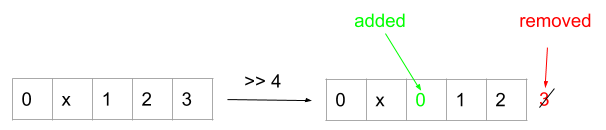
\includegraphics[width=0.6\linewidth]{sprint4/bitshift-illustration.png}
    \caption{Right bit shifting a hexadecimal by 4 bits.}
    \label{fig:sprint4-bit-shift-basic}
\end{figure}
This can be utilized to read the different parts of the message that the client received.
The first part that is read from the message is timestamp.
In the message the decimals representing the timestamp are followed by two decimals representing the type of the message as seen earlier.
Because one digit corresponds to four bits, the message has to be right bit shifted by 8 bits to move the timestamp to the back of the hexadecimal as illustrated on \autoref{fig:sprint4-bitshift-timestamp}.
\begin{figure}[H]
    \centering
    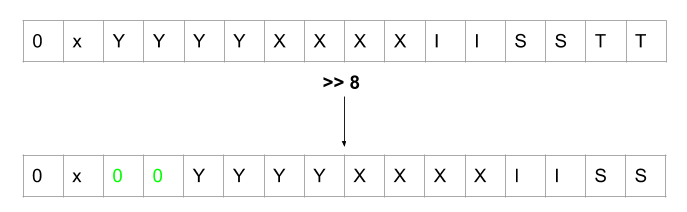
\includegraphics[width=0.6\linewidth]{sprint4/bitshift-timestamp-illustration.png}
    \caption{Right bitshifting the message by 8 bits to get the timestamp to the back.}
    \label{fig:sprint4-bitshift-timestamp}
\end{figure}

The message can then be typecasted to a \texttt{byte} to extract the timestamp from the package.
The next part that is read from the message is the player id.
Decimals representing the player id are followed by four decimals representing the timestamp and the type of the package.
This means that to get the player id to the back of the hexadecimal the message has to be right bit shifted by 16 bits.
\begin{figure}[H]
    \centering
    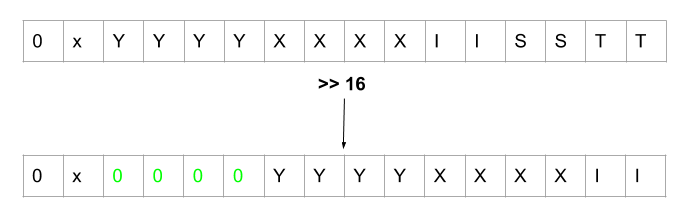
\includegraphics[width=0.6\linewidth]{sprint4/bitshift-playerid-illustration.png}
    \caption{Right bitshifting the message by 16 bits to get the player id to the back.}
    \label{fig:sprint4-bitshift-playerid}
\end{figure}
Because the player id is represented as two decimals it can be decoded from the message by typecasting the message to the \texttt{byte} datatype in C\#.
This is done for each part of the message where the message is right bitshifted by the combined size of the previously read parts and then typecasted to a datatype that has the same size as the part of the message that is being read.
\subsection*{TCP client}
The principle behind the TCP client is much like the UDP client, where the type is read as a byte and then a switch statement ensures that the data is handled by the correct function.
However, since TCP is sent as a stream, all packages have been prefixed with a numerical values to indicate the length of each package.
This means that the client cannot simply wait for a new message, read it and act according to the type.
Instead, the client will read the first two bytes of the stream and then read the incoming amount of bytes indicated by this numerical value, allowing the program to handle packages of varying length.
